% ------------------------------------------------------------------------
% -*-TeX-*- -*-Hard-*- Smart Wrapping
% ------------------------------------------------------------------------
\def\baselinestretch{1}

\chapter{Methodology Design}

\def\baselinestretch{1.44}

%%% ----------------------------------------------------------------------

This chapter outlines the methodology developed for my dissertation project. 
   
\smallskip

%%% ----------------------------------------------------------------------
\goodbreak
\section{Analysis of the methods}
The core hypothesis of this study is that MultiTaskLassoCV, will outperform single-task learning (LassoCV) in both accuracy and robustness. By applying an L1-norm regularization, LassoCV penalizes the absolute size of coefficients, encouraging sparsity in the model, which can enhance interpretability. However, while LassoCV is effective for single-task learning, it might not fully exploit the inherent relationships between different mental health indicators in schizophrenia \citep{tibshirani1996regression}. MultiTaskLassoCV extends LassoCV to a multi-task framework, allowing simultaneous training across multiple related tasks. This approach is particularly advantageous in the context of mental health prediction, where symptoms are often interrelated. By leveraging these relationships, MultiTaskLassoCV is anticipated to yield superior performance in predicting schizophrenia-related mental health conditions, both in terms of accuracy and robustness (\citep{zhou2011malsar} and \citep{tseng2020using}). 

For a given user's data~\(X_{u} \in \mathbb{R}^{e_{u} \times d}\) and the EMA symptom scores \(Y_u^s \in \mathbb{R}^{e_{u}}\)  the objective is shown below: 

\[\min_{W_u^s} \| Y_u^s - X_u W_u^s \| + \alpha | W_u^s|_{1}\] u represents the user, \(e_{u}\)  represents the number of EMA entries by the user, d is the feature vector dimension, s is the symptom and  \(\alpha\) controls the sparsity of \(w_u^s\), higher \(\alpha\) values result in fewer non-zero coefficients.

The weight vector is represented by : \(w_u^s \in \mathbb{R}^d\) and it's used for predicting symptom s for user u, while the \(l_{1}\)-norm\(|W_u^s|_{1}\) = \sum{i}\ |w_{ui}^s|

The magnitude of these coefficients indicates the importance of each feature in predicting EMA scores. However, for the generalized model where a single model is used to predict all the users, the objective function is shown below : 

\[\min_{W^s} \| Y^s - X W^s \| + \alpha | W^s|_{1}\] where
\(X =[X_{1} & \cdots & X_{p} ]\in \mathbb{R} ^{(\sum_{u=1}^{p} e_u\ )}\) denotes the combined feature matrix for users 1,2,3 to
p and \(Y^s =[Y^s_{1} & \cdots & Y^s_{p} ]\in \mathbb{R} ^{(\sum_{u=1}^{p} e_u\ )\times d}\) denotes combined EMA scores for symptom s across all patients and \(w_u^s \in \mathbb{R}^d\), which is the weight vector.

For multi-task learning, a given user's EMA scores across various symptoms is represented as \(Y_u = [Y^1_{u} & \cdots & Y^k_{u} ] \in \mathbb{R}^{eu \times k}\) 
where k denotes the total number of symptoms. The objective function for MTL is defined based on the approaches outlined by \citet{nie2010efficient} and  \citet{zhou2011malsar} as shown below :
\[\min_{W_u} \| Y_u - X_u W_u \|_F^2 + \alpha \| W_u \|_{2,1}\]


\(W_u = [W^1_{u} & \cdots & W^k_{u} ]\in \mathbb{R}^{d \times k} \) serves as the weight matrix used for predicting individual symptom scores. The regularization parameter is denoted by \(\alpha\), and \(||.||_F\) represents the Frobenius norm. \(.|| W ||_{2,1}\)  term is calculated as \(\sum\_{i}  \sqrt{\sum_{j} w^2_{i\j} }\) reflecting  \(l_{2,1}\)-norm, which is effective in promoting joint group sparsity by encouraging related tasks to share a limited set of features \citep{tseng2020using}.

 Generalized modeling for both auto selection and hyperparameter tuning for Single-Task Learning (STL) and Multi-Task Learning (MTL) were examined. For personalized modeling, sufficient data is crucial, which is a limitation of this dataset. To confirm the assumption regarding data sufficiency, personalized modeling was performed, and the results from participants with the highest and lowest number of entries—study\_id 47 and study\_id 70, respectively—were evaluated. This selection was used to compare the performance of STL and MTL approaches across all symptoms. Due to computational constraints, only the automatic feature selection using LassoCV and MultitaskLassoCV were evaluated.
 
 The decision to use MultitaskLassoCV and LassoCV over alternatives like Ridge regression, ElasticNet, or other multi-task learning methods, is based on its ability to promote joint sparsity and improve prediction accuracy in high-dimensional settings, which is critical for the nuanced detection of schizophrenia-related conditions.


\section{Design of Methodology}
This section outlines the steps taken to prepare, ensuring robust and reliable model development.
\subsection {Data Exploratory Analysis and Visualization} 
\subsubsection{Data Source} 
The data used for this study was provided by my supervisor Dr.Min Aung, who was part of the team that carried out the CrossCheck research \citep{wang2016crosscheck}, ensuring compliance with ethical standards and data privacy regulations. The dataset spans January 21, 2015, to April 20, 2017.

\subsubsection{Data Features} 
The dataset comprises 155 features across 23,573 rows, including behavioral metrics divided into four six-hour intervals each day to capture daily patterns. The features include 57 numeric (float) features, 97 numeric (integer) features and 1 categorical feature. The data includes key behavioral metrics such as conversation frequency, movement activities (e.g., vehicle, bike, foot), and self-reported Ecological Momentary Assessment (EMA) scores, which are critical for understanding the mental health states of the participants as shown in Figure \ref{feat} and Table 3.1

\begin{figure}[H]
    \centering
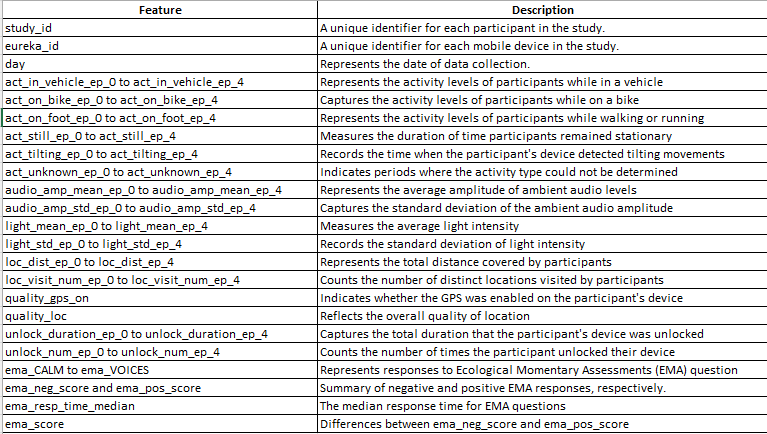
\includegraphics[scale=0.50]{feature.png}
\caption{Data Features}
\label{feat}
\end{figure}

\bigskip
\goodbreak
    
\smallskip
\begin{table}[H]
\centering
\caption{ 10 EMA questions as extracted from \citet{wang2016crosscheck}}
\begin{tabular}{|l|}
\hline
\textbf{Questions} \\ \hline
Have you been feeling CALM? \\ \hline
Have you been SOCIAL? \\ \hline
Have you been bothered by VOICES? \\ \hline
Have you been SEEING THINGS other people can’t see? \\ \hline
Have you been feeling STRESSED? \\ \hline
Have you been worried about people trying to HARM you? \\ \hline
Have you been SLEEPING well? \\ \hline
Have you been able to THINK clearly? \\ \hline
Have you been DEPRESSED? \\ \hline
Have you been HOPEFUL about the future? \\ \hline
\textbf{Options:} 0- Not at all; 1- A little; 2- Moderately; 3- Extremely. \\ \hline
\end{tabular}
\end{table}

\smallskip
 \subsubsection{Descriptive Statistics } 
Descriptive statistics was implemented to assess the variability in participants' activities and the EMA. Correlation analysis was conducted to explore the relationships between different (EMA) scores and other variables. Outliers were detected using the z-score method, and a thorough analysis of missing values was performed to identify features with incomplete data. Additionally, the consistency of aggregated scores was verified by ensuring that the sum of scores for epochs 1 through 4 matched the total score for epoch 0.


\subsection{Data Cleaning} 
The `Eureka\_id` column was excluded as it has no impact on the analysis. In addition, all aggregated features (e.g., `epoch\_0`) were excluded from the dataset due to mismatched aggregated scores to enhance the data quality.  The refined dataset now comprises 126 features and 12,232 observations, ensuring a robust foundation for analysis.
 \subsubsection{Handling Missing Values}
To handle missing values in targets which are the 10 symptoms, backfilling was applied with a limit of three days as the EMA questions and responses were gotten within 2 to 3 days. Interpolation and removal of remaining missing values were also examined, in addition to mean imputation and removal of rows with missing values for other variables. Among all the methods evaluated, backfilling missing EMA values within a three-day window and subsequently removal of outstanding missing data method was adopted for the data cleaning as it performed better. This observation aligns with the assumptions made by \citet{adler2020predicting}, who suggest that interpolation methods can introduce bias by smoothing data towards mean values. This bias may obscure subtle variations in the data, thereby limiting the ability of models to accurately identify changes indicative of mental health status.
\subsubsection{Handling Outliers}
Outliers, particularly in the "day" column, were addressed by removing data that fell outside the study period (e.g., entries from 1969), which likely resulted from device configuration errors.
\subsection{Feature engineering}
In the crosscheck dataset, different columns such as audio\_conversations, location\_distance, sms\_in,call\_duration have varying scales.Using these features without normalizing them to a uniform scale could introduce bias into the model. The StandardScaler was applied for feature standardization, ensuring all features contribute equally to the model, preventing any single feature from disproportionately influencing the results due to its scale. This is particularly useful for linear regression algorithms like LassoCV that are sensitive to the scale of the input features \citep{mayer1974procedures} and \citep{mathur2023generalized}

 \subsubsection{Cross-Validation}
Cross-validation is a pivotal component in refining the LassoCV model, particularly for schizophrenia prediction. This method involves partitioning the dataset into \( k \) subsets, known as folds, allowing the model to be trained and validated systematically. The process is repeated \( k \) times, with each fold serving once as the validation set and the remaining \( k-1 \) folds as the training set. This iterative approach not only aids in identifying the optimal regularization parameter, \(\alpha\), but also ensures a model that strikes a balance between accurately fitting the training data and generalizing to new, unseen data \citep{kolluri2020reducing}

In the context of schizophrenia research, where overfitting can result in misleading conclusions, cross-validation enhances model reliability and predictive power, especially when forecasting Ecological Momentary Assessment (EMA) outcomes. Furthermore, integrating an 80-20\% data split with cross-validation adds an extra layer of validation: after the model is optimized on 80\% of the data using cross-validation, the remaining 20\% serves as a hold-out set, providing an independent test of the model’s performance on entirely new data. This study also explored hyperparameter tuning for the \(\alpha\) value, comparing manually tuned results with those automatically selected by LassoCV. This comparison underscores LassoCV's robust framework for developing predictive models, highlighting its potential to optimize predictive accuracy and clinical utility. 

\section{Evaluation Methods and Measures}
In mental health, large prediction errors can have serious implications. For example, underestimating the severity of a patient's condition might lead to inadequate care, while overestimating it might result in unnecessary interventions. RMSE's sensitivity to large errors ensures that models are penalized more for these significant mistakes, promoting the development of models that minimize these critical errors. The RMSE value is in the same unit as the outcome being predicted. This is particularly important in mental health, where clinicians and stakeholders often need to understand model performance in practical, understandable terms. In addition, mental health data often involves significant variability due to individual differences in symptom presentation and response to treatment. RMSE’s penalization of variance in errors helps ensure that the model does not produce predictions with wide variability, which could lead to inconsistent or unreliable assessments. This is crucial in mental health, where consistency in evaluation is vital for accurate diagnosis and treatment planning. Also,mental health datasets can include outliers, such as extreme cases of severe mental health conditions. RMSE's sensitivity to these outliers ensures that the model does not ignore or overly smooth out these critical cases. In mental health, where extreme cases often need more attention, having an evaluation metric that highlights poor performance in these areas is beneficial. Using RMSE as an evaluation metric for mental health datasets is justified due to its ability to highlight significant errors, maintain interpretability, and manage variability in predictions. In the context of Schizophrenia,  where accurate prediction and consistency are paramount, RMSE helps ensure that models perform reliably across a range of cases, including those with extreme outcomes. This makes RMSE a valuable tool for evaluating and improving predictive models in mental health research and practice \citet{zhang2024students}.

To test for the significance of the difference between the STL and MTL were examined using the Wilcoxon test. The Wilcoxon test was selected for comparison because it is a non-parametric test, meaning it does not require the assumption of normality in the dataset. Additionally, it is ideal for comparing the performance of STL and MTL models on the same set of targets, and it is well-suited for small sample sizes \citep{tseng2020using}


\section{Tools and Resources}
The research was conducted using a variety of tools and resources that supported efficient data processing and accurate analysis. They include :
\begin{itemize}
    \item Programming Languages: Python was the primary language used due to its robust data science libraries and widespread adoption in machine learning.
    \item Libraries and Frameworks: Pandas and NumPy were used for data manipulation and processing. Scikit-learn was employed for implementing machine learning algorithms and conducting model evaluations. Matplotlib and Seaborn facilitated detailed data visualizations, important for understanding data distributions and model outcomes.
   \item Development Environments: Although Jupyter Notebook and Google Colab were used as they provide an interactive environment for coding and visualization, Google Colab was chosen for its cloud-based computing capabilities, enabling efficient handling of computationally intensive tasks and providing access to GPU acceleration when needed.
   \item Data Resources: The dataset was provided by my supervisor, ensuring its relevance and quality, tailored specifically to the research objectives.
\end{itemize}

These tools and resources were instrumental in ensuring the smooth execution of the project, from data preprocessing to model evaluation

\section{Summary} 
This chapter outlined the methodology used to evaluate the hypothesis of this study that      MultiTaskLassoCV would outperform LassoCV in detecting schizophrenia-related mental health symptoms. The analysis of methods highlighted the advantages of MultiTaskLassoCV in handling complex, multifaceted data. The design of the methodology detailed the steps taken to prepare the data, including exploratory analysis, data preprocessing, and feature engineering. RMSE evaluation metrics was chosen to balance precision and interpretability, while the tools and resources section underscored the critical role of Python, Scikit-learn, and various visualization libraries.

   

\def\baselinestretch{1.66}
\medskip

%%% ----------------------------------------------------------------------
